\subsection{Space charge: from a KV beam to particle tracking}
\label{sec:space-charge}
A proton beam repels itself. The electric self-force pushes particles away from
the beam centre and reduces the restoring force of the magnets. Consequently,
the transverse oscillations usually slow down: their tunes decrease with beam
current. This section derives an analytic prediction and compares it with an
OPALX simulation of the same 16-cell lattice. The analytic model explains the
mechanism; the particle calculation tests the approximations.

Here $s$ denotes arc length along the \emph{magnetic closed orbit}, rather than
along the placement circle in Eq.~\eqref{eq:circle}. Local $x$ is horizontal and
normal to that orbit, and $y$ is vertical. These lower-case coordinates describe
displacements from the orbit. A prime denotes differentiation with respect to
$s$. The paraxial approximation assumes small transverse slopes, $|x'|,|y'|\ll1$.
We first assume fixed energy, uncoupled transverse motion and a long beam with
negligible longitudinal self-force.

\subsubsection{Which current sets the strength of space charge?}
For protons of rest mass $m$ and charge $q>0$, define
\begin{equation}
 \gamma=1+\frac{T}{mc^2},\qquad
 \beta=\frac{v}{c}=\sqrt{1-\gamma^{-2}},\qquad
 I=\lambda\beta c.
 \label{eq:sc-current}
\end{equation}
The line-charge density $\lambda$ has units C/m. A uniformly populated bunch
of full length $L_b$ and total charge $\mathcal Q_b$ has
\begin{equation}
 \lambda=\frac{\mathcal Q_b}{L_b},\qquad
 \mathcal Q_b=\frac{I L_b}{\beta c},\qquad
 \overline I=\frac{\mathcal Q_b}{T_{\rm rev}}
            =I\frac{L_b}{C_{\rm co}},
 \label{eq:sc-bunch-charge}
\end{equation}
where $C_{\rm co}$ is the closed-orbit length and $T_{\rm rev}=C_{\rm co}/(\beta c)$.
The current $I$ is the current \emph{inside the bunch}; $\overline I$ is the
current averaged over a revolution for one bunch. They are different when
most of the ring is empty. Local transverse space charge depends on $I$.

At 12 MeV, $\beta=0.15842$, $\gamma=1.01279$ and
$C_{\rm co}\simeq28.0297$ m. For $L_b=0.20$ m, a bunch current of 10.399 mA
therefore requires only 43.793 pC; its revolution-averaged current is about
$74.2\ \mu$A. When comparing this short FFA bunch with a longer bunch in a
different lattice, we keep the \emph{bunch current} fixed, not the total charge.

\subsubsection{What is special about the KV distribution?}
The Kapchinskij--Vladimirskij (KV) distribution is an idealized transverse
phase-space distribution whose projection into position space is a uniformly
charged ellipse.\footnote{I.~M.~Kapchinskij and V.~V.~Vladimirskij,
``Limitations of proton beam current in a strong focusing linear accelerator
associated with the beam space charge,'' in the 1959 CERN conference proceedings,
p.~274 ff., especially Sections II--IV;
\href{https://s3.cern.ch/inspire-prod-files-5/526fe2f2ff6f05063bcb9a9b08da12f9}{original paper}.}
Its usefulness follows from that uniform density: the electric field inside
the ellipse is linear in displacement.

For either plane $j=x,y$, the rms emittance and Twiss parameters describe the
second moments about the beam centroid:
\begin{equation}
 \begin{aligned}
 \varepsilon_j&=\sqrt{\langle j^2\rangle\langle j'^2\rangle
                         -\langle jj'\rangle^2},\\
 \Sigma_j&=\begin{pmatrix}\langle j^2\rangle&\langle jj'\rangle\\
                 \langle jj'\rangle&\langle j'^2\rangle\end{pmatrix}
 =\varepsilon_j\begin{pmatrix}\beta_j^{\rm Tw}&-\alpha_j^{\rm Tw}\\
                 -\alpha_j^{\rm Tw}&\gamma_j^{\rm Tw}\end{pmatrix},
 \qquad \gamma_j^{\rm Tw}=\frac{1+(\alpha_j^{\rm Tw})^2}{\beta_j^{\rm Tw}}.
 \end{aligned}
 \label{eq:sc-twiss}
\end{equation}
The superscript ``Tw'' distinguishes the optical functions from the relativistic
factors $\beta$ and $\gamma$. The brackets denote an average over particles,
with the centroid subtracted. The geometric rms emittance $\varepsilon_j$ has
units m\,rad; the normalized rms emittance is
$\varepsilon_{n,j}=\beta\gamma\varepsilon_j$ at fixed energy.

For each current, use its matched Twiss parameters and rms emittances to
introduce dimensionless normalized coordinates,
\begin{equation}
 u_j=\frac{j}{\sqrt{\varepsilon_j\beta_j^{\rm Tw}}},\qquad
 v_j=\frac{\alpha_j^{\rm Tw}j+\beta_j^{\rm Tw}j'}
              {\sqrt{\varepsilon_j\beta_j^{\rm Tw}}}.
 \label{eq:sc-normalized}
\end{equation}
A KV beam samples the \emph{surface} of a four-dimensional sphere:
\begin{equation}
 f_{\rm KV}\ \propto\
 \delta\!\left(u_x^2+v_x^2+u_y^2+v_y^2-4\right).
 \label{eq:sc-kv-shell}
\end{equation}
Thus it is not a uniformly filled four-dimensional ball and not a Gaussian.
Integrating over the two momentum coordinates gives a uniform position density
inside an ellipse. Its edge semi-axes $a,b$ are twice the rms sizes:
\begin{equation}
 a=2\sigma_x,\qquad b=2\sigma_y,\qquad
 \rho(x,y)=\frac{\lambda}{\pi a b}
 \quad\hbox{for}\quad \frac{x^2}{a^2}+\frac{y^2}{b^2}\leq1,
 \label{eq:sc-kv-density}
\end{equation}
with zero density outside. Mixing edge radii and rms sizes gives incorrect
space-charge factors. All emittances in this section are \emph{rms} emittances.

\subsubsection{Linear self-forces and the envelope equations}
In free space, the transverse electric field inside that ellipse is
\begin{equation}
 E_x=\frac{\lambda}{\pi\epsilon_0}\frac{x}{a(a+b)},\qquad
 E_y=\frac{\lambda}{\pi\epsilon_0}\frac{y}{b(a+b)}.
 \label{eq:sc-kv-field}
\end{equation}
For a round beam, $a=b$, this reduces to
$E_r=\lambda r/(2\pi\epsilon_0 a^2)$, as obtained directly from Gauss's law.
The beam current also produces a magnetic self-field. For particles moving
approximately together, its inward force partially cancels the electric force:
\begin{equation}
 \vect B_{\rm sc}=\frac{\beta}{c}\,\vect t\times\vect E_\perp,\qquad
 \vect F_\perp\simeq q(1-\beta^2)\vect E_\perp
                   =\frac{q}{\gamma^2}\vect E_\perp.
 \label{eq:sc-cancellation}
\end{equation}
Here $\vect t$ is the orbit tangent. The electric repulsion dominates, so the
net self-force remains defocusing.

The dimensionless generalized perveance collects the current and energy
scaling:
\begin{equation}
 K=\frac{2I}{I_A\beta^3\gamma^3},\qquad
 I_A=\frac{4\pi\epsilon_0mc^3}{q}
      \simeq31.30\times10^6\ \mathrm{A}\quad\hbox{for protons}.
 \label{eq:sc-perveance}
\end{equation}
The proton value must be used here, not the much smaller electron value.
Dividing the transverse force by $m\gamma\beta^2c^2$ converts it to an
acceleration with respect to $s$. If $\kappa_x(s)$ and $\kappa_y(s)$ denote
the external linear focusing functions, the particle equations become
\begin{equation}
 \begin{aligned}
 x''+[\kappa_x(s)-g_x(s)]x&=0,&g_x&=\frac{2K}{a(a+b)},\\
 y''+[\kappa_y(s)-g_y(s)]y&=0,&g_y&=\frac{2K}{b(a+b)}.
 \end{aligned}
 \label{eq:sc-particle}
\end{equation}
Both $\kappa_j$ and $g_j$ have units m$^{-2}$. The positive $g_j$ reduces the
external focusing. For a KV distribution, its rms envelopes obey
\begin{equation}
 \boxed{\begin{aligned}
 \sigma_x''+\kappa_x\sigma_x-\frac{\varepsilon_x^2}{\sigma_x^3}
                   -\frac{K}{2(\sigma_x+\sigma_y)}&=0,\\
 \sigma_y''+\kappa_y\sigma_y-\frac{\varepsilon_y^2}{\sigma_y^3}
                   -\frac{K}{2(\sigma_x+\sigma_y)}&=0.
 \end{aligned}}
 \label{eq:sc-envelopes}
\end{equation}
The four terms describe envelope curvature, external focusing, emittance
pressure and space-charge defocusing. For example, multiplying the horizontal
equation by two and substituting $a=2\sigma_x$ gives an emittance term
$16\varepsilon_x^2/a^3$ and a space-charge term $2K/(a+b)$ in the edge-radius
equation. This provides a useful check on conventions.

\subsubsection{Matching the beam and predicting its tunes}
A matched beam breathes with the periodic lattice, but repeats its envelope
and envelope slope after one cell. With cell length $\ell_c=C_{\rm co}/16$,
the matching conditions are
\begin{equation}
 \sigma_j(s+\ell_c)=\sigma_j(s),\qquad
 \sigma_j'(s+\ell_c)=\sigma_j'(s).
 \label{eq:sc-match}
\end{equation}
To find a matched beam at a chosen current, keep the two emittances fixed and
adjust the initial sizes and correlations until these conditions hold. Reusing
the zero-current sizes without rematching would generally excite envelope
oscillations and complicate the tune comparison.

Our analytic calculation uses linear transfer maps obtained by differentiating
the magnetic equations about the verified closed orbit. It alternates these
external maps with short KV defocusing kicks. In slope coordinates a kick of
length $\Delta s$ in either plane is
\begin{equation}
 L_j=\begin{pmatrix}1&0\\g_j\Delta s&1\end{pmatrix},\qquad
 \Sigma_j\longmapsto L_j\Sigma_jL_j^{\mathsf T}.
 \label{eq:sc-kick}
\end{equation}
The actual calculation uses mechanical momenta normalized by $mc$ and transforms
the radial reference-section coordinates to the local orbit-normal frame.
In that momentum convention $p_x/(mc)\simeq\beta\gamma x'$, so the lower-left
kick element includes an additional factor $\beta\gamma$. The physical force
is the same. Half kicks on both sides of each external map give a symmetric
integration. Iterating the covariance to periodicity implements
Eq.~\eqref{eq:sc-match}; this is an analytic-field model solved numerically,
not a fit to the OPALX tune measurements.

Let $M_{j,c}$ be the resulting matched one-cell particle matrix in plane $j$.
For stable uncoupled motion, its eigenvalues are $\exp(\pm i\mu_j)$, with
\begin{equation}
 \cos\mu_j=\tfrac12\operatorname{Tr}M_{j,c},\qquad
 Q_j=\frac{16\mu_j}{2\pi},\qquad
 \Delta Q_j(I)=Q_j(I)-Q_j(0).
 \label{eq:sc-tunes}
\end{equation}
The phase branch is followed continuously from the zero-current solution.
The tune counts \emph{particle oscillations per revolution}; it is not the
frequency of the centroid or the envelope. In the weak-space-charge limit,
first-order optics gives the useful estimate
\begin{equation}
 \Delta Q_j\simeq-\frac{1}{4\pi}
       \oint\beta_{j,0}^{\rm Tw}(s)g_j(s)\,\mathrm ds.
 \label{eq:sc-perturbation}
\end{equation}
The minus sign explains tune depression. The full matched calculation also
allows the envelope and therefore $g_j$ to change with current.

\subsubsection{What OPALX calculates with FFT2D5}
OPALX follows individual macroparticles in the nonlinear magnetic fields
introduced in Section~2. A macroparticle represents many protons: with
$N_{\rm mac}$ equal-weight particles its deposited charge is
$\mathcal Q_b/N_{\rm mac}$, while the tracked charge-to-mass ratio remains the
proton value. The distribution can deform during tracking; OPALX does not
force it to remain KV or enforce linear self-fields.

The FFT2D5 solver uses a \emph{particle-in-cell} method. It resolves the charge
on a three-dimensional mesh, but solves a two-dimensional transverse Poisson
problem for each longitudinal slice. This is the meaning of ``2.5D.'' It is
a local, long-beam approximation, rather than a full three-dimensional Poisson
solution. For this study the sequence is:
\begin{enumerate}
 \item Project each particle onto the supplied closed reference path and form
 local transverse coordinates and an arc-length coordinate $s$.
 \item Deposit macroparticle charges with cloud-in-cell weights. For constant
 timestep and longitudinal cloud-in-cell deposition, the density has the form
 \begin{equation}
  \rho_{ijk}=\frac{1}{\Delta x\Delta y\Delta s}
       \sum_p q_p W_i(x_p)W_j(y_p)W_k(s_p),
  \label{eq:sc-cic}
 \end{equation}
 where each linear weight $W$ connects neighbouring cell centres and the
 weights for a particle sum to one.
 \item In each occupied slice $k$, solve
 \begin{equation}
  \left(\partial_x^2+\partial_y^2\right)\Phi_k
        =-\frac{\rho_k}{\epsilon_0},\qquad
  \vect E_{\perp,k}=-\nabla_\perp\Phi_k.
  \label{eq:sc-poisson}
 \end{equation}
 The solver evaluates the free-space logarithmic Green-function convolution
 with fast Fourier transforms (FFTs). It doubles the transverse computational
 domain for the convolution and integrates the Green function over a mesh
 cell, including the singular self-cell. Finite differences of the potential
 give the electric field. FFTs accelerate this calculation; they do not impose
 a conducting transverse wall.
 \item Interpolate the field back to particles with the corresponding
 cloud-in-cell weights. Construct the transverse magnetic self-field as in
 Eq.~\eqref{eq:sc-cancellation} and rotate both fields back to the laboratory.
 The transverse Poisson source already uses charge per \emph{laboratory}
 length, so its electric field is already the laboratory field; applying
 another factor $\gamma$ would double-count a transformation.
 \item Add the external magnetic fields and advance the relativistic Lorentz
 equations with the Boris integrator:
 \begin{equation}
  \frac{\mathrm d\vect r}{\mathrm dt}=\frac{\vect p}{m\gamma_p},\qquad
  \frac{\mathrm d\vect p}{\mathrm dt}
       =q\left[\vect E_{\rm sc}+\vect v\times
                       (\vect B_{\rm ext}+\vect B_{\rm sc})\right],
  \quad\gamma_p=\sqrt{1+\frac{|\vect p|^2}{m^2c^2}}.
  \label{eq:sc-lorentz}
 \end{equation}
 The setting \texttt{SCFIELDUPDATE=MIDPOINT} evaluates the collective field at
 the midpoint stage of the time step.
\end{enumerate}
In this scan, \texttt{PIPEMODE=NONE} disables the approximate longitudinal
space-charge field: $E_s^{\rm sc}=0$. Transverse space charge remains active.
The bunch ends therefore do not generate longitudinal self-forces in this
model. The parameters \texttt{PIPESIZEX} and \texttt{PIPESIZEY} set the transverse
mesh widths; they do not specify conducting-wall boundary conditions for this
transverse free-space solve. With \texttt{CLOSEDRING=TRUE}, the longitudinal
coordinate wraps around the closed reference path.

\subsubsection{The school scan and its numerical resolution}
The zero-current launch has radial rms size 5.0 mm and vertical rms size
2.4 mm at the $Z=0$ reference section. The horizontal size here is a radial
section measurement; the KV self-force uses the size after transformation to
the local orbit-normal plane. The geometric rms emittances are approximately
26.338 and 3.748 mm\,mrad, or normalized rms emittances 4.226 and
0.6014 mm\,mrad. Matching at each nonzero current changes the sizes slightly
while keeping the emittances fixed. Each 20 cm bunch contains 98,304
macroparticles. The source uses 128 uniformly spaced longitudinal midpoint
slices and a symmetric, low-noise sample of the KV shell in each slice.
These source slices and the field-mesh slices are distinct discretizations.

The transverse field grid has $64\times64$ cells across
$64\times64$ mm, so $\Delta x=\Delta y=1$ mm. The longitudinal grid spans the
\emph{entire} reference path, including the empty part of the ring. Its spacing
and the number of cells occupied by the bunch are approximately
\begin{equation}
 \Delta s=\frac{C_{\rm co}}{N_s},\qquad
 N_{s,\rm bunch}=\frac{L_b}{\Delta s}
      =\frac{L_bN_s}{C_{\rm co}}.
 \label{eq:sc-grid}
\end{equation}
Choosing $N_s=17920$ gives $\Delta s=1.564$ mm and about 128 cells across
20 cm. Setting the full-ring value to $N_s=128$ would instead give
$\Delta s=21.9$ cm, leaving less than one cell across the bunch. That would
smear the line density and underestimate the local self-force.

The time step is 50 ps. Short pilot comparisons checked particle IDs, finite
coordinates, charge, one versus two GPU ranks, and 50 versus 25 ps steps.
The latter comparison gives a maximum position difference of $0.276\ \mu$m
after 25 ns. These are useful implementation checks, but do not establish
long-time tune convergence. The target record is 128 turns; the preliminary
comparison below uses the same first 15 turns in every case.

\begin{table}[ht]
\centering
\caption{School intensity scan. The current is the current inside the uniform
20 cm bunch. The KV tunes come from the periodic linear self-field model.}
\begin{tabular}{@{}rrrr@{}}
\toprule
$I$ [mA] & $\mathcal Q_b$ [pC] & $Q_{x,\rm KV}$ & $Q_{y,\rm KV}$\\
\midrule
0      & 0      & 3.410660 & 3.391112\\
4.749  & 19.998 & 3.408404 & 3.385117\\
8.701  & 36.643 & 3.406527 & 3.380131\\
10.399 & 43.793 & 3.405722 & 3.377991\\
\bottomrule
\end{tabular}
\label{tab:sc-scan}
\end{table}

\subsubsection{Reading the tune footprint and its colour bar}
A tune footprint places one point $(Q_x,Q_y)$ for each analysed particle.
We estimate the tunes with Numerical Analysis of Fundamental Frequencies
(NAFF), using position records resampled at equal azimuth intervals and a
Hann window of order two. The horizontal closed-orbit scalloping is removed
before interpolation; the central-slice centroid is removed to measure
incoherent particle tunes. All four cases use 768 corresponding particles
from the central longitudinal slice and the same 15-turn interval, starting
one-quarter turn after launch. Corresponding particles have the same
normalized launch directions; matching changes their physical coordinates
slightly as the current increases.

The colour identifies how each particle initially shares its \emph{normalized}
transverse action between the two planes. Define the Courant--Snyder action
and its dimensionless version by
\begin{equation}
 \mathcal I_j=\frac{\gamma_j^{\rm Tw}j^2+2\alpha_j^{\rm Tw}jj'
                         +\beta_j^{\rm Tw}j'^2}{2},\qquad
 \frac{\mathcal I_j}{\varepsilon_j}=\frac{u_j^2+v_j^2}{2}.
 \label{eq:sc-actions}
\end{equation}
The KV shell fixes the sum of the normalized actions to two. The horizontal
fraction used by the colour bar is therefore
\begin{equation}
 \boxed{f_x=
 \frac{\mathcal I_x/\varepsilon_x}
      {\mathcal I_x/\varepsilon_x+\mathcal I_y/\varepsilon_y}
 =\frac{u_x^2+v_x^2}{4},\qquad 0\leq f_x\leq1.}
 \label{eq:sc-colour}
\end{equation}
Dark purple, near $f_x=0$, denotes particles with predominantly vertical
normalized oscillation amplitude. Yellow, near $f_x=1$, denotes predominantly
horizontal normalized amplitude. At $f_x=0.5$, the two normalized actions are
equal. The corresponding ratios can be read directly:
\begin{equation}
 \frac{\mathcal I_x}{\varepsilon_x}=2f_x,\qquad
 \frac{\mathcal I_y}{\varepsilon_y}=2(1-f_x).
 \label{eq:sc-colour-examples}
\end{equation}
For example, $f_x=0.75$ means normalized actions 1.5 horizontally and 0.5
vertically: a ratio of three to one. It does \emph{not} mean that the horizontal
position is three times the vertical position. Position also depends on
oscillation phase and optical functions. Because the two emittances differ,
equal normalized actions do not mean equal actions in physical units, equal
amplitudes in millimetres, or equal transverse kinetic energies.

The colours are \emph{initial labels}. The same label is used for corresponding
particles at every current. In the ideal matched linear KV model the actions
are invariants. In the nonlinear FFA fields, these initial linear actions need
not stay constant. A colour trend across a footprint shows the dependence of
the measured tunes on the initial action sharing; it is not a time sequence,
a current scale, or a density scale. The red crosses mark analytic KV tunes
and are not assigned a value on the colour bar. The linear KV model predicts
one tune pair for the matched core, whereas finite-amplitude magnetic motion
and a nonideal self-field can produce a footprint.

\begin{figure}[htbp]
\centering
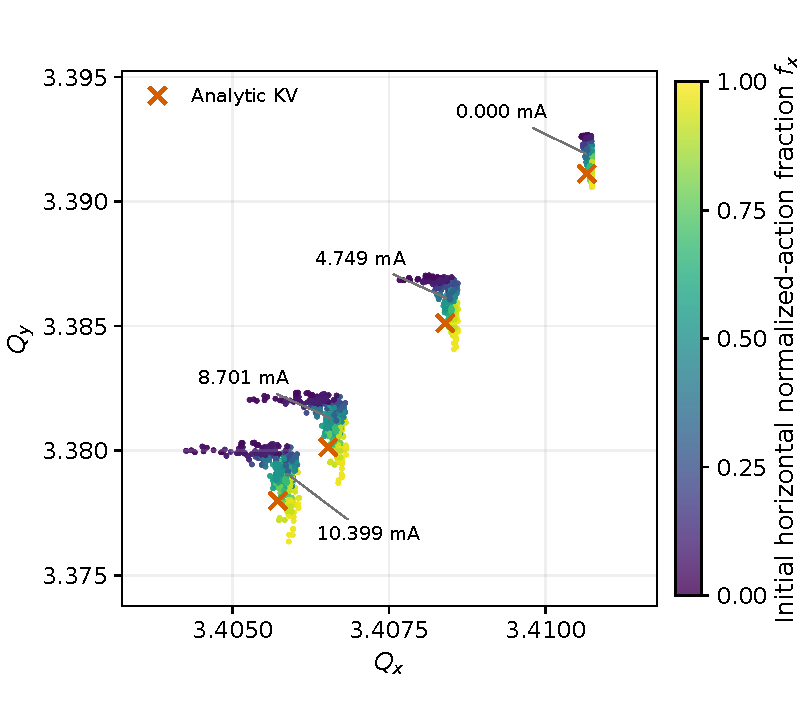
\includegraphics[width=.76\textwidth]{figures/tune-footprint.pdf}
\caption{Preliminary FFA tune footprints at bunch currents 0, 4.749, 8.701 and
10.399 mA, labelled next to their particle clouds. Each cloud contains NAFF
tunes from 768 central-slice particles over the same 15 turns; red crosses are
the corresponding analytic KV predictions. The colour bar gives the
\emph{initial horizontal normalized-action fraction}
$f_x=(u_x^2+v_x^2)/4$: purple means mainly vertical action, yellow mainly
horizontal action, and $f_x=0.5$ equal normalized actions. It does not encode
current or charge. The four clouds shift towards smaller tunes with current;
the zero-current cloud already has a finite-amplitude spread.}
\label{fig:sc-footprint}
\end{figure}

\subsubsection{Comparing the tune shifts fairly}
To isolate the intensity dependence, subtract each method's own zero-current
baseline:
\begin{equation}
 \begin{aligned}
 \Delta Q_{j,\rm NAFF}(I)&=
   \operatorname{median}_p Q_{j,p}(I)
       -\operatorname{median}_p Q_{j,p}(0),\\
 \Delta Q_{j,\rm KV}(I)&=Q_{j,\rm KV}(I)-Q_{j,\rm KV}(0).
 \end{aligned}
 \label{eq:sc-baseline}
\end{equation}
This definition is a difference of medians, which need not equal the median
of the per-particle differences. It also removes the offset between the
finite-amplitude zero-current particle median and the linear zero-amplitude
KV prediction. That offset is about $7.35\times10^{-4}$ vertically in the
present short record.

\clearpage
\begin{figure}[htbp]
\centering
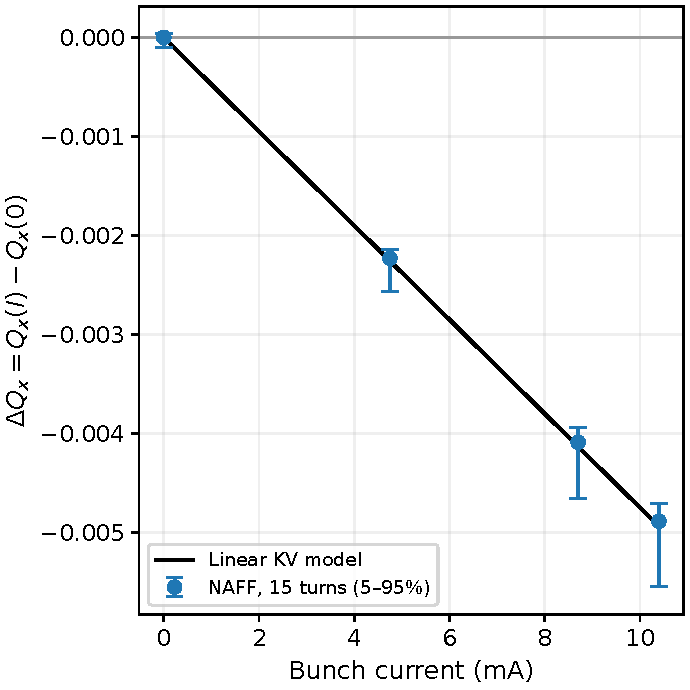
\includegraphics[width=.49\textwidth]{figures/preliminary-dQx.pdf}\hfill
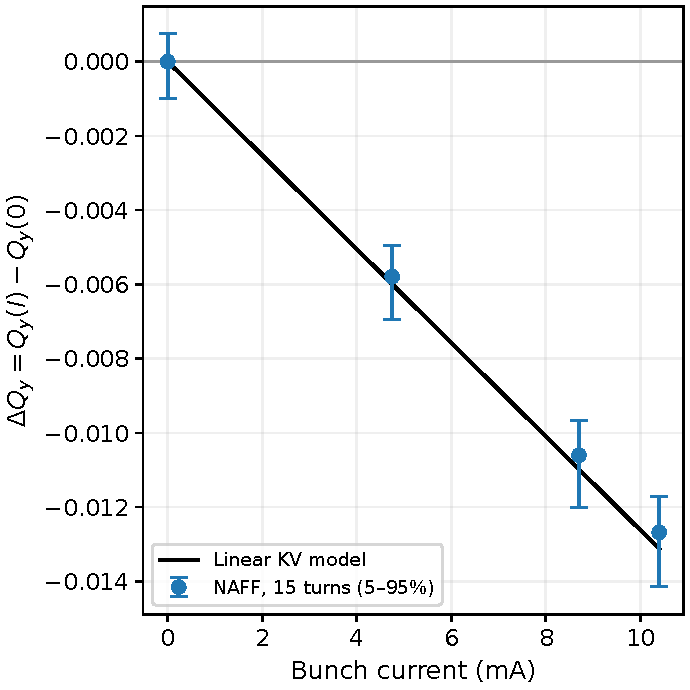
\includegraphics[width=.49\textwidth]{figures/preliminary-dQy.pdf}
\caption{Preliminary tune shifts relative to each method's own zero-current
baseline, for the same 15-turn records and central-slice particles as
Fig.~\ref{fig:sc-footprint}. Dots are differences of NAFF median tunes; black
curves connect the matched linear KV predictions. Bars give the 5th--95th
percentile particle footprint at each current, shifted by the zero-current
median. They are \emph{not} uncertainty bars on the median or a distribution
of paired-particle tune differences. The NAFF and KV results show similar
tune depression in both planes.}
\label{fig:sc-shifts}
\end{figure}

At 10.399 mA the median-based shifts are approximately
$\Delta Q_x=-0.004886$ and $\Delta Q_y=-0.012680$, compared with KV values
$-0.004939$ and $-0.013122$. The simulated depressions are about 1.1\% and
3.4\% smaller in magnitude. This is an encouraging preliminary trend, not
a percent-level accuracy result. Changing the NAFF record from 11 to 15 turns
changes individual tunes by up to $7.6\times10^{-5}$ horizontally and
$3.9\times10^{-4}$ vertically at the 95th percentile. A short-window estimate
can move when several stationary spectral lines overlap; that alone does
not demonstrate a changing fundamental tune or chaotic diffusion.

Before assigning the residual difference to a physical mechanism, compare
longer records, check the tune footprint against record length, and test
particle number, field-grid resolution and timestep. The KV model assumes
linear external focusing and a uniform elliptical density with no
longitudinal self-force. OPALX retains nonlinear external fields and evolves
a finite macroparticle distribution on a mesh, while using the same
longitudinal-force approximation here. These distinctions explain what the
comparison tests, without identifying a cause for the remaining discrepancy.
